\documentclass[pdftex,12pt,a4paper]{report}
\usepackage[pdftex]{graphicx}
\usepackage{caption}
\usepackage{subcaption}
%% \usepackage{wrapfig}
\newcommand{\HRule}{\rule{\linewidth}{0.5mm}}
\usepackage[italian]{babel}
\usepackage{indentfirst}
\usepackage{enumerate} % permette di scegliere il tipo di elenco
                       % (lettere, numeri arabi, romani..)
\usepackage[margin=1in]{geometry} % margini stretti

\usepackage{alltt} % tipo verbatim ma accetta comandi tipo \emph{...}

\usepackage{amsmath} % \eqref{}

%% custom chapters
\usepackage{titlesec}
%% Questo stampa 1. Nomecapitolo, invece che
%% Capitolo 1.
%% Nomecapitolo
\titleformat{\chapter}{\normalfont\huge\bfseries}{\thechapter.}{20pt}{\huge}

\usepackage{amssymb}
\usepackage{latexsym}

\usepackage{amsthm}
\theoremstyle{plain}
\newtheorem{teo}{Teorema}[chapter] % mettendo section conta i teoremi
                                % con #capitolo.#sezione.#teorema
                                % mentre con chapter #cap.#teo
\newtheorem{prop}[teo]{Proposizione}
\newtheorem{cor}[teo]{Corollario}
\newtheorem{lemma}[teo]{Lemma}
\theoremstyle{definition}
\newtheorem{defn}{Definizione}[chapter]
\theoremstyle{remark}
\newtheorem{oss}{Osservazione}[chapter]
\newtheorem{notaz}{Notazione}[chapter]
\newtheorem{ex}{Esempio}[chapter]

%% \usepackage{showkeys} % toglimi!

\graphicspath{ {./images/} }

\begin{document}
\begin{titlepage}
\begin{center}

% Upper part of the page. The '~' is needed because \\
% only works if a paragraph has started.

\includegraphics[width=0.30\textwidth]{stemma}~\\[1cm]

\textsc{\LARGE Universit\`a degli Studi Firenze}\\[1.5cm]

\LARGE Scuola di Scienze Matematiche, Fisiche e Naturali\\
\LARGE C.d.L in Matematica\\[0.5cm]

\Large Anno accademico 2011-2012\\
\Large Relazione finale per la Laurea Triennale\\[1.5cm]

% Title
%% \HRule \\[0.4cm]
{ \huge \bfseries Young Tableaux: una implementazione}\\[1.0cm]
{ \LARGE \bfseries Young Tableaux: an implementation}\\[0.4cm]
%% \HRule \\[1.5cm]


\vspace{4cm}

% Bottom of the page

% Author and supervisor
\begin{minipage}{0.4\textwidth}
\begin{flushleft} \large
\emph{Candidato:}\\
Alessandro \textsc{Campagni}
\end{flushleft}
\end{minipage}
\begin{minipage}{0.4\textwidth}
\begin{flushright} \large
\emph{Relatore:} \\
Prof. Marco \textsc{Maggesi}
\end{flushright}
\end{minipage}

\end{center}
\end{titlepage}

\chapter{Preliminari}

\section{Diagrammi e tabelle}

\begin{defn}[Diagramma di Young]
Un diagramma di Young $\lambda=(n_1,n_2,\dots,n_k)$ \`e una
rappresentazione di una partizione di un intero positivo $n =
\sum_{i=0}^{k}{n_i}$ come somma di interi positivi $n_k \geq \ldots \geq
n_2 \geq n_1 \geq 0$. Graficamente possiamo immaginare un diagramma di
Young come $k$ righe di celle quadrate, allineate a sinistra, di
lunghezza $n_k,\ldots,n_2,n_1$ dall'alto verso il basso in quest'ordine.
\end{defn}

\begin{defn}[Diagramma coniugato]
Dato un diagramma di Young $\lambda=(n_1,n_2,\dots,n_k)$, definiamo il
suo coniugato $\tilde{\lambda}$ come il diagramma che ha le colonne di
lunghezza $n_k,\ldots,n_2,n_1$ da sinistra verso destra in quest'ordine.  
\end{defn}

\begin{figure}[h]
\centering

\begin{subfigure}[b]{0.4\textwidth}
\centering
\includegraphics[height=0.35\textwidth]{YoungDiagram}
\caption{$\lambda=(1,1,2,3,4)$}
%% \label{fig:awesome_image}
\end{subfigure}%
\begin{subfigure}[b]{0.4\textwidth}
\centering
\raisebox{0.2\height}{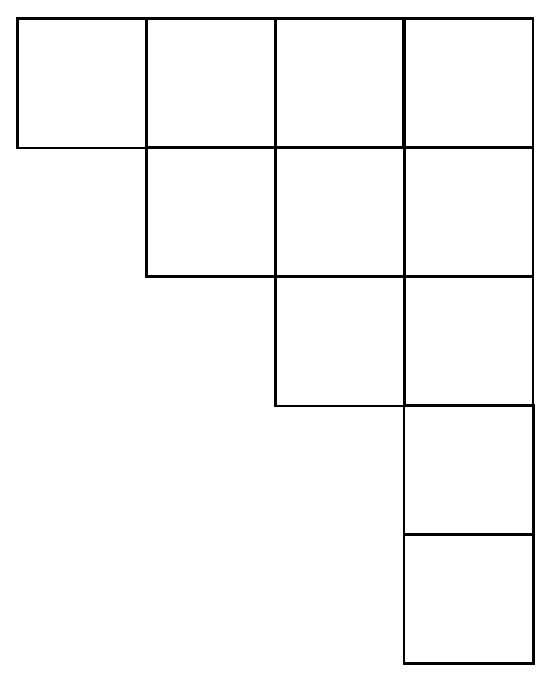
\includegraphics[height=0.35\textwidth,angle=90]{YoungDiagramFlip}}
\caption{$\tilde{\lambda}=(1,2,3,4)$}
\end{subfigure}
\caption{Un diagramma di Young ed il suo coniugato.}
\end{figure}

Possiamo calcolare il diagramma coniugato con la funzione
\emph{ydiagram\_transpose\_rows}:

\begin{alltt}
\emph{remove\_diagram\_column} (r, l) := 
if emptyp (r) then return (l)
else block (
  l : append ([length (r)], l),
  r : r-1,
  r : delete (0, r),
  return (\emph{remove\_diagram\_column} (r, l)));

\emph{ydiagram\_transpose\_rows} (d) := \emph{remove\_diagram\_column} (d, []);
\end{alltt}

La funzione \emph{remove\_diagram\_column} toglie la colonna pi\`u a
sinistra del diagramma e la inserisce come ultima riga del diagramma coniugato.

\begin{notaz}
Scriveremo $\lambda \vdash n$ intendendo che $\lambda$ \`e una
partizione di $n$.
\end{notaz}

\begin{defn}
Diremo che un diagramma $\mu=(n_1,n_2,\dots,n_k)$ \emph{\`e pi\`u
piccolo} di un diagramma $\lambda=(m_1,m_2,\dots,m_h)$, e scriviamo
$\mu \subset \lambda$, se
\begin{enumerate}[(i)]
\item $k \leq h$;
\item $n_i \leq m_i$ per ogni $1 \leq i \leq k$.
\end{enumerate}
\end{defn}

\begin{defn}[Skew diagram]
Uno skew diagram \`e il diagramma che si ottiene togliendo a
diagramma di Young $\lambda$ un diagramma pi\`u piccolo $\mu \subset
\lambda$. Indicheremo lo skew diagram cos\`i ottenuto con $\lambda / \mu$.
\end{defn}

\begin{defn}[Tabella di Young]\label{ytab}
Diremo Young tableau un riempimento di un diagramma di Young con
numeri interi positivi che risulti:
\begin{enumerate}[(i)]
\item non decrescente lungo le righe;
\item strettamente crescente lungo le colonne.
\end{enumerate}
Un Young tableau si dice \emph{standard} se il riempimento di
$\lambda \vdash n$ \`e composto dai primi $n$ interi positivi (non
ripetuti).
\end{defn}

\begin{oss}
Un Young tableau standard \`e strettamente crescente \emph{anche}
lungo le righe.
\end{oss}

\begin{oss}
Ogni tabella $T$ \`e riempimento di un unico diagramma $\lambda$. Il
diagramma di cui $T$ \`e riempimento \`e detto \emph{forma di $T$}
\end{oss}

\begin{defn}[Skew tableau]
Diremo skew tableau un riempimento di uno skew diagram che rispetti i
requisiti della definizione \ref{ytab}. 
\end{defn}

\section{Row bumping}
Il row bumping \`e la procedura con la quale dati un tableau $T$ e un
intero positivo $x$ si costruisce un tableau, che indicheremo con $T
\gets x$, la cui forma ha un box in pi\`u della forma di $T$ con
entrata $x$.\\
Se $x_1 = x$ \`e non minore di ciascun elemento della prima riga
dall'alto di $T$, aggiungiamo alla fine di tale riga l'entrata x.
Altrimenti se $x_2$ \`e il primo elemento da sinistra della prima riga
di $T$ strettamente maggiore di $x_1$, inseriamo $x_1$ al posto di
$x_2$ e procediamo al suo inserimento nella seconda riga di $T$.
Ripetiamo quindi per le successive righe, fino a quando non siamo in
grado di effettuare un inserimento al termine di una riga oppure fino
a quando aggiungeremo una riga in basso contenente l'elemento $x_h$
sostituito nell'ultima riga al passo precedente con l'elemento
$x_{h-1}$.

La funzione \emph{rec\_bump\_row} effettua il row bumping di un dato
elemento $x$ in una riga $r$ scorrendola dal fondo (chiameremo infatti
la funzione con $i$ pari alla lunghezza della riga) fino a trovare
l'elemento da sostituire oppure aggiungendo una nuova entrata in coda.
Restituisce la riga modificata con, eventualmente, l'elemento da
inserire nella riga successiva.

La funzione \emph{rec\_ytableau\_word\_bump} esegue il row bumping
fino a quando \`e possibile, e se necessario aggiunge una nuova riga
al tableau.

\begin{alltt}
\emph{rec\_bump\_row} (r, x, i) :=
if (x >= last (r)) then [append (r, [x]), 0]
else if ((i > 0) and (x < r[i])) then \emph{rec\_bump\_row} (r, x, i-1)
else block (
  [next\_x],
  next\_x : r[i+1],
  r[i+1] : x,
  return ([r, next\_x]));

\emph{rec\_ytableau\_word\_bump} (t, x, i) :=
if (x > 0) then block (
  [],
  if (i > 0) then block (
    [next\_b],
    next\_b : \emph{rec\_bump\_row} (t[i], x, length (t[i])),
    t[i] : next\_b[1],
    return (\emph{rec\_ytableau\_word\_bump} (t, next\_b[2], i-1)))
  else return (append ([[x]], t)))
else t;
\end{alltt}

\begin{figure}[h]
\centering
\includegraphics[width=0.8\textwidth]{row_bump}
\caption{Row bumping}
\end{figure}

\begin{oss}
Al termine di ogni iterazione della funzione
\emph{rec\_ytableau\_word\_bump} la variabile $t$ \`e la parola di un
tableau. In particolare la funzione \emph{rec\_ytableau\_word\_bump}
restituisce uno Young tableau.
%% \begin{proof}
%% Infatti la funzione \emph{rec\_bump\_row} restituisce una lista
%% ordinata in modo non decrescente (da sinistra verso destra), che
%% quindi rispetta la prima propriet\`a della definizione \ref{ytab}.\\
%% Supponiamo ora che al termine di una certa iterazione smetta di valere la seconda
%% propriet\`a, ovvero stiamo inserendo nella posizione
%% $(i,j)$ un intero $x$ minore o uguale dell'elemento $\bar{x}$ in
%% posizione $(i-1,j)$.\\
%% Durante l'iterazione precedente si \`e quindi inserito $y$ al posto di
%% $x$ nella riga $(i-1)$-esima, e poich\`e $x \leq \bar{x}$ tale
%% inserimento deve essere avvenuto (per la (i) della definizione
%% \ref{ytab}) in posizione $(i-1,k)$, con $k \leq j$. Sia $x_0$
%% l'elemento in posizione $(i,k)$, allora $x < x_0$.\\
%% Siamo quindi giunti ad un assurdo, infatti un tale inserimento
%% contraddice la non decrescenza. 
%% \end{proof}
\end{oss}

Iterando l'operazione di row bumping si ha la seguente

\begin{defn}
Dati due tableaux $T$ e $U$, dette $x_1,\ldots , x_s$ le entrate di
$U$ da sinistra verso destra e dal basso verso l'alto, definiamo
$T \cdot U = (( \ldots ((T \gets x_1) \gets x_2 ) \gets \ldots ) \gets x_{s-1} )
\gets x_s$.
\end{defn} 

\begin{oss}
Il prodotto di tableaux non \`e commutativo, infatti ad esempio
\begin{center}
\includegraphics[width=0.3\textwidth]{prod_non_comm_oneline}
\end{center}
\end{oss}

\section{Algebra dei tableaux}

\begin{prop}\label{tableaux_monoid}
L'insieme dei tableaux con l'operazione di prodotto \`e un monoide con
unit\`a il tableau vuoto $T \cdot \varnothing = \varnothing \cdot T = T$.
\end{prop}

La dimostrazione di questo fatto richiede l'introduzione di alcuni
concetti.

\begin{defn}[Parola]
Dato un tableau o uno skew tableau $T$, diciamo row word, word o parola
di $T$, che indicheremo con $w(T)$, la parola che si ottiene elencando
da sinistra verso destra, dal basso verso l'alto le entrate di $T$.

\begin{notaz}
Se $u$ e $v$ sono due parole, scriviamo $u \leq v$ intendendo che
\emph{ogni} lettera di $u$ \`e minore o uguale ad \emph{ogni} lettera
di $v$.
\end{notaz}

\begin{alltt}
\emph{word\_from\_ytableau} (l, t) :=
if (not emptyp (t)) then \emph{word\_from\_ytableau} (append (l, t[1]), rest (t, 1))
else l;
\end{alltt}
\end{defn}

\begin{oss}
Dalla parola $w(T)$ di un tableau \`e possibile risalire al tableau
$T$ osservando che le righe di $T$, dal basso verso l'alto, si
ottengono leggendo la parola da sinistra verso destra e interrompendo
ogni volta in cui una lettera \`e strettamente minore della
precedente.
\begin{alltt}
\emph{ytableau\_from\_word} (l,t) :=
if ((not emptyp (l)) and (not emptyp (t))) then block (
  if (last (t[1])) <= l[1] then block (
    t[1] : append (t[1], [l[1]]),
    return (\emph{ytableau\_from\_word} (rest (l, 1), t)))
  else block (
    t : append ([[l[1]]], t),
    return (\emph{ytableau\_from\_word} (rest (l, 1), t))))
else if (not emptyp (l)) then block (
  t : [[l[1]]],
  return (\emph{ytableau\_from\_word} (rest (l, 1), t)))
else reverse (t);
\end{alltt}
\end{oss}

La cosa interessante \`e l'effetto del row bumping sulla
parola di un tableau. 
Possiamo interpretare l'algoritmo che descrive
il row bumping in termini di parole: sia $w = w(T)$ la parola in questione e
$x$ l'elemento da inserire. Possiamo fattorizzare $w=\bar w \cdot u \cdot \bar x \cdot
v$ dove $\bar w$ \`e la parola del tableau ottenuto da $T$ rimuovendo
la prima riga e $u \cdot \bar x \cdot v$ \`e la parola corrispondente
alla prima riga di $T$, dove $u$ \`e composta da lettere non maggiori
di $x$ e $\bar x > x$. Si ha $w \cdot x = \bar w \cdot \bar x \cdot u \cdot x
\cdot v$. Cio\`e:

\begin{equation}\label{row_bump_word}
(u \cdot \bar x \cdot v) \cdot x \rightsquigarrow \bar x \cdot u \cdot
  x \cdot v \mbox{ se } u \leq x < \bar x \leq v
\end{equation}

Ora se $v=v_1 \ldots v_k$ la \eqref{row_bump_word}, tenuto conto che
$x < \bar x \leq v_i$ per ogni $1 \leq i \leq k$, diventa

\begin{equation}\label{pre_bump}
\begin{split}
u \cdot \bar x \cdot v_1 \cdot \ldots \cdot v_k \cdot x
\rightsquigarrow u \cdot \bar x \cdot v_1 \cdot \ldots \cdot v_{k-1}
\cdot x \cdot v_k \rightsquigarrow \ldots\\
\ldots \rightsquigarrow u \cdot \bar x \cdot v_1 \cdot \ldots \cdot
v_i \cdot x \cdot v_{i+1} \cdot \ldots \cdot v_k \rightsquigarrow \ldots
\rightsquigarrow u \cdot \bar x \cdot x \cdot v_1 \cdot \ldots \cdot v_k
\end{split}
\end{equation}

inoltre detto $u=u_1 \ldots u_h$, dato che $u_i \leq x < \bar x$, possiamo
descrivere il bumping di $\bar x$ come

\begin{equation}\label{bump}
\begin{split}
u_1 \cdot \ldots \cdot u_k \cdot \bar x \cdot x \cdot v
\rightsquigarrow u_1 \cdot \ldots \cdot u_{h-1} \cdot \bar x \cdot u_k
\cdot x \cdot v \rightsquigarrow \ldots\\
\ldots \rightsquigarrow u_1 \cdot \ldots \cdot u_i \cdot \bar x \cdot
u_{i+1} \cdot \ldots u_h \cdot x \cdot v \rightsquigarrow \ldots
\rightsquigarrow \bar x \cdot u_1 \cdot \ldots \cdot u_h \cdot x \cdot v.
\end{split}
\end{equation}

Possiamo quindi identificare due trasformazioni fondamentali: la prima
viene applicata ad ogni passaggio in \eqref{pre_bump}, la seconda
viene applicata in \eqref{bump}:

\begin{equation}\label{k1}\tag{$K_1$}
y \cdot z \cdot x \rightsquigarrow y \cdot x \cdot z \mbox{ se } x < y
\leq z
\end{equation}
\begin{equation}\label{k2}\tag{$K_2$}
y \cdot z \cdot x \rightsquigarrow z \cdot y \cdot x \mbox{ se } y
\leq x < z
\end{equation}

\begin{defn}[Trasformazione elementare di Knuth]
Una trasformazione di una parola si dice elementare di Knuth se
applica a tre lettere consecutive la trasformazione \eqref{k1},
\eqref{k2} o una delle loro inverse.
\end{defn}

\begin{defn}[Knuth-equivalenti]
Due parole $w$ e $w'$ si dicono Knuth-equivalenti, e si scrive $w
\equiv w'$ se \`e possibile ottenere una dall'altra, e viceversa, per
mezzo di sole trasformazioni elementari di Knuth.
\end{defn}
%% \newpage % tornava brutto con l'immagine alla pagina dopo
\begin{oss}
Le trasformazioni fondamentali \eqref{k1} e \eqref{k2} sono coerenti
con il row bumping, infatti

\begin{figure}[h]
\centering

\begin{subfigure}[b]{0.3\textwidth}
\centering
\includegraphics[height=0.2\textwidth]{KnuthK1}\\
\eqref{k1} $x < y \leq z$
%% \label{fig:awesome_image}
\end{subfigure}%
\begin{subfigure}[b]{0.3\textwidth}
\centering
\includegraphics[height=0.2\textwidth]{KnuthK2}\\
\eqref{k2} $y \leq x < z$
\end{subfigure}

\caption{Trasformazioni fondamentali}
\end{figure}
\end{oss}

\begin{prop}\label{word_bump_equiv}
Siano $T$ un tableau e $x$ un intero positivo, allora $w(T \gets x) = w(T)
\cdot x$. In particolare, dato un altro tableau $U$ si ha $w(T\cdot U)
= w(T) \cdot w(U)$.
\end{prop}

Data una parola $w = x_1 \ldots x_k$ possiamo sempre costruire un
tableau, per mezzo di quella che viene detta \emph{procedura canonica}
calcolando $T = (( \ldots ((\varnothing \gets x_1) \gets x_2 ) \gets \ldots ) \gets x_{k-1} )
\gets x_k$. Il tableau ottenuto ha parola $w(T)$ Knuth-equivalente a
$w$.

\begin{teo}\label{knuth_equiv_word}
Ogni parola \`e Knuth-equivalente alla parola di un unico tableau.
\end{teo}

Osservando che la giustapposizione di parole \`e associativa, si ha
infine la proposizione \ref{tableaux_monoid}.

\chapter{Polinomi di Schur}

\begin{defn}[Polinomio di Schur]
Data una partizione $\lambda \vdash n$ (i.e. un diagramma di Young
$\lambda = (n_1, \ldots, n_m)$) in $m$ parti (e quindi il diagramma ha
$m$ righe) e un qualunque tableau $T$ che riempie $\lambda$ indichiamo
con $x^T = \prod\limits_{i = 1}^m x^{c(i)}$. Sommando al variare di
$T$ fra i possibili riempimenti di $\lambda$ otteniamo
\begin{math}
s_\lambda(x_1,\ldots,x_m) = \sum x^T
\end{math}
che chiameremo polinomio di Schur.
\end{defn}

\section{Anello dei tableau}

Sia $W_{[m]}$ l'insieme delle parole sull'alfabeto $[m]$ e sia
$\sim_K$ la relazione di Knuth-equivalenza. $M_{[m]} =
\frac{W_{[m]}}{\sim_K}$ \`e l'insieme delle classi di equivalenza,
definiamo in $M_{[m]}$ un'operazione di prodotto attraverso la giustapposizione di parole e
osseriviamo che \`e ben definito, infatti se $v \sim_K v'$ e $u \sim_K
u'$ si ha $v \cdot u \sim_K v' \cdot u \sim_K v \cdot u'$. In
definitiva $(M, \cdot, \varnothing)$, dove $\varnothing$ \`e la
parola vuota, \`e un monoide che, per il
teorema \eqref{knuth_equiv_word}, possiamo identificare con il monoide
dei tableaux.

Il monoide $M$ ha un anello associato (dettagli su Algebra
S.Lang) che chiameremo \emph{anello dei tableaux}, e indicheremo con
$R_{[m]}$ e che \`e uno $\mathbb{Z}$-modulo libero generato dai
tableaux ad entrate in $[m]$ con prodotto il prodotto di tableaux.
Resta quindi definito un omomorfismo
\begin{equation}
\begin{matrix}\label{ring_tab}
\psi: & R_{[m]} & \rightarrow  & \mathbb{Z}[x_1,\ldots,x_m]\\
& T      & \mapsto & \psi(T)=x^T
\end{matrix}
\end{equation}
Indichiamo con $S_\lambda[m] \in R_{[m]}$ la somma di tutti i tableaux
che riempiono il diagramma $\lambda$, allora
$\psi(S_\lambda[m])=s_\lambda(x_1,\ldots,x_m)$ \`e il polinomio di
Schur corrispondente alla partizione $\lambda$ con $m$ variabili.

\section{Implementazione dei polinomi di Schur}

\begin{alltt}
\emph{yschur\_monomial\_word\_recursive} (flat\_w, mon, i) := block (
  [x],
  if (i>0) then return (\emph{yschur\_monomial\_word\_recursive} (flat\_w,
                                                        mon*x[flat\_w[i]],
                                                        i-1))
  else return (mon));

\emph{last\_or\_zero} (l) := if emptyp (l) then 0 else last(l);

\emph{fill\_next\_line} (len, m, prev, ls) := block (
  [],
  if (len = 0) then return (ls)
  else block (
    [p],
    p : [],
    for x in ls do p : append (p,
                               makelist (append (x, [y]),
                               y,
                               max (\emph{last\_or\_zero} (x) + 1,
                                    prev[length (x)+1]),
                               m - len + 1)),
    return (\emph{fill\_next\_line} (len - 1, m, prev, p))));


\emph{fl\_fill\_line} (len, m, ls) :=
if (len=0) then ls
else \emph{fl\_fill\_line} (len-1, m, xreduce ('append, 
                                       makelist (makelist (append (x, [y]),
                                                 y,
                                                 \emph{last\_or\_zero} (x) + 1,
                                                 m - len +1), x,
                                                 ls)));

\emph{fl\_list\_transposed\_ytableaux} (shape, level, m, ts) :=
if level < length (shape) then
  if level > 0 then
    if not emptyp (flatten (ts)) then block (
      [nls,ts\_first],
      ts\_first : first (ts),
      ts : delete (ts\_first, ts),
      nls : \emph{fill\_next\_line} (shape [level+1], m,
                            rest (ts\_first, -length(ts\_first)+shape[level]),
                            [[]]),
      ts : append (ts, map (lambda ([x], append (x, ts\_first)), nls)),
      if every (lambda ([x],
                        is (length (flatten (x)) = length (flatten
                        (first (ts))))),
                ts) then level : (level + 1),
      \emph{fl\_list\_transposed\_ytableaux} (shape, level, m, ts))
    else []
  else \emph{fl\_list\_transposed\_ytableaux} (shape, level + 1, m,
                                     \emph{fl\_fill\_line} (shape[level + 1], m, ts))
else ts;

\emph{fl\_better\_yschur\_polynomial} (d, m) := block (
  [ts, pol, shape],
  shape : reverse ((\emph{ydiagram\_transpose} (d))@rows),
  print (shape),
  ts : \emph{fl\_list\_transposed\_ytableaux} (shape, 0, m, [[]]),
  pol : 0,
  for i : 1 thru length (ts) do
    pol : pol + \emph{yschur\_monomial\_word\_recursive} (ts[i], 1, length (ts[i])),
  return (pol));
\end{alltt}

Il cuore dell'algoritmo risiede nella funzione
\emph{fl\_list\_transposed\_ytableaux} che calcola tutti i
possibili tableaux su un dato diagramma $\lambda$. Dal momento che la
definizione \eqref{ytab} pone una condizione
lungo le colonne pi\`u stringente della non decrescenza sulle
righe, calcoliamo i possibili riempimenti del diagramma coniugato
$\tilde{\lambda}$, cos\`i facendo gi\`a dalla prima riga (ovvero la
prima colonna di $\lambda$) riduciamo il numero di riempimenti da
provare.\\
Il riempimento della prima riga avviene da sinistra verso destra
attingendo da $[m]=\{1,\ldots, m\}$ in modo tale che se inseriamo $k \in
[m]$ in posizione $i$-esima, e la prima riga \`e lunga $l_1$, esistano
$k_1,\ldots,k_{l_1-1} \in [m]$ tutti maggiori di $k$. Generiamo quindi
una lista di possibili riempimenti della prima riga, ognuno dei quali
dar\`a luogo ad una lista di possibili riempimenti delle prime due
righe, e cos\`i via.\\ 
Naturalmente riempiendo la riga $j$-esima, alla
posizione $i$ dovremo scegliere $k \in [m]$ tale che esistano
$k_1,\ldots,k_{l_j-1} \in [m]$ tutti maggiori di $k$ e tutti non
minori dell'elemento in posizione $i$-esima della riga
$(j-1)$-esima.\\
Ottenuta infine la lista dei possibili tableaux su $\lambda$ la
funzione \emph{yschur\_monomial\_word\_recursive} calcola il
corrispondente monomio, la somma di questi monomi \`e il polinomio di
Schur cercato $s_\lambda(x_1,\ldots,x_m)$.

% Non sono sicuro di doverne parlare. Per ora lascio in sospeso.
%% \section{Corrispondenza di Robinson-Schensted-Knuth}
%% Data una parola $w=x_1\ldots x_r$ indichiamo con $P(w)$ l'\emph{unico} tableau con
%% parola Knuth-equivalente a $w$ (teorema \eqref{knuth_equiv_word}). Un
%% modo per ottenede $P(w)$ data $w$ \`e la \emph{procedura canonica}
%% vista nel capitolo precedente. Mentre costruiamo il tableau $P(w)$
%% teniamo traccia delle posizioni in cui stiamo inserendo le lettere di
%% $w$ costruendo un'altra tabella $Q(w)$ della stessa forma di $P(w)$
%% inserendo $k$ in posizione $Q(w)^i_j$ ogniqualvolta inseriamo $x_k$
%% nella riga $i$-esima alla colonna $j$-esima del tableau $P(w)$. Dunque
%% se stiamo costruendo $P_k=P(x_1\ldots x_k)=P_{k-1} \gets x_k =
%% ((\ldots (\varnothing \gets x_1) \gets \ldots ) \gets x_{k-1} ) \gets
%% x_k$ inseriremo $k$ in $Q_k=Q(x_1 \ldots x_k)$ in corrispondenza della posizione
%% presente in $P_k$ ma non in $P_{k-1}$.

%% \begin{oss}
%% Ad ogni passo $1 \leq k \leq r$ della procedura canonica, $Q_k$ \`e un
%% tableau standard.
%% %% \begin{proof}
%% %% Chiaramente le entrate di $Q(w)$ sono tutte distinte fra loro essendo
%% %% indici delle lettere della parola $w$. Supponiamo che $Q_k$ sia un
%% %% tableau standard, si hanno tre casi:\\
%% %% $x_k < x_{k+1}$: \\
%% %% $x_k = x_{k+1}$:\\
%% %% $x_k > x_{k+1}$:\\
%% %% \end{proof}
%% \end{oss}

%% Essendo note le posizioni in cui sono state inserite le varie lettere,
%% da $(P(w),Q(w))$ possiamo ricostruire $w$, questo significa che data
%% una qualunque coppia di tableaux $(P,Q)$ che riempiono lo stesso
%% diagramma con $Q$ standard esiste una parola $\bar w$ tale che
%% $(P,Q)=(P(\bar w),Q(\bar w))$.\\
%% Abbiamo cos\`i una corrispondenza
%% biunivoca fra le lettere $w$ di lunghezza $r$ con lettere
%% nell'alfabeto $[n]$ e le coppie $(P,Q)$ di tableaux riempimenti dello
%% stesso diagramma $\lambda \vdash r$ con $P$ ad entrate in $[n]$ e $Q$
%% standard. Nel caso particolare in cui $r=n$ e le lettere di $w$ siano
%% tutte diverse una dall'altra, ovvero $w \in S_n$, si ha che anche $P$
%% \`e uno standard tableau e viceversa.

\chapter{Regola di Littlewood-Richardson}
% Non sono sicuro di doverne parlare. Per ora lascio in sospeso.
\section{Corrispondenza di Robinson-Schensted-Knuth}\label{RSKcorr}
Data una parola $w=x_1\ldots x_r$ indichiamo con $P(w)$ l'\emph{unico} tableau con
parola Knuth-equivalente a $w$ (teorema \ref{knuth_equiv_word}). Un
modo per ottenede $P(w)$ data $w$ \`e la \emph{procedura canonica}
vista nel capitolo precedente. Mentre costruiamo il tableau $P(w)$
teniamo traccia delle posizioni in cui stiamo inserendo le lettere di
$w$ costruendo un'altra tabella $Q(w)$ della stessa forma di $P(w)$
inserendo $k$ in posizione $Q(w)^i_j$ ogniqualvolta inseriamo $x_k$
nella riga $i$-esima alla colonna $j$-esima del tableau $P(w)$. Dunque
se stiamo costruendo $P_k=P(x_1\ldots x_k)=P_{k-1} \gets x_k =
((\ldots (\varnothing \gets x_1) \gets \ldots ) \gets x_{k-1} ) \gets
x_k$ inseriremo $k$ in $Q_k=Q(x_1 \ldots x_k)$ in corrispondenza della posizione
presente in $P_k$ ma non in $P_{k-1}$.

\begin{oss}
Ad ogni passo $1 \leq k \leq r$ della procedura canonica, $Q_k$ \`e un
tableau standard.
%% \begin{proof}
%% Chiaramente le entrate di $Q(w)$ sono tutte distinte fra loro essendo
%% indici delle lettere della parola $w$. Supponiamo che $Q_k$ sia un
%% tableau standard, si hanno tre casi:\\
%% $x_k < x_{k+1}$: \\
%% $x_k = x_{k+1}$:\\
%% $x_k > x_{k+1}$:\\
%% \end{proof}
\end{oss}

Essendo note le posizioni in cui sono state inserite le varie lettere,
da $(P(w),Q(w))$ possiamo ricostruire $w$, questo significa che data
una qualunque coppia di tableaux $(P,Q)$ che riempiono lo stesso
diagramma con $Q$ standard esiste una parola $\bar w$ tale che
$(P,Q)=(P(\bar w),Q(\bar w))$.

Abbiamo cos\`i una corrispondenza
biunivoca fra le parole $w$ di lunghezza $r$ con lettere
nell'alfabeto $[n]$ e le coppie $(P,Q)$ di tableaux riempimenti dello
stesso diagramma $\lambda \vdash r$ con $P$ ad entrate in $[n]$ e $Q$
standard. Nel caso particolare in cui $r=n$ e le lettere di $w$ siano
tutte diverse una dall'altra, ovvero $w \in S_n$, si ha che anche $P$
\`e uno standard tableau e viceversa.

\begin{notaz}[Vettore doppio]
Chiamiamo vettore doppio una matrice $2 \times n$. 
\end{notaz}

\begin{defn}
Un vettore doppio
\begin{math}
\begin{bmatrix}
u_1 & \ldots & u_m\\
v_1 & \ldots & v_m
\end{bmatrix}
\end{math}
si dice in ordine lessicografico se valgono:
\begin{enumerate}[(i)]
\item $u_1 \leq \ldots \leq u_n$;
\item $v_i \leq v_{i+1}$ se $u_1 = u_{i+1}$.
\end{enumerate}
\end{defn}

Knuth generalizz\`o (per i dettagli si veda ~\cite{fulton1997young})
la corrispondenza precedente ad una qualunque coppia di
tableau $(P,Q)$, che riempiono lo stesso diagramma, con $P$ ad entrate
in $[n]$ e $Q$ in $[m]$. In questo caso si ha la corrispondenza fra le
coppie $(P,Q)$ e i \emph{vettori doppi} in ordine lessicografico
\begin{math}
\begin{bmatrix}
u_1 & \ldots & u_m\\
v_1 & \ldots & v_m
\end{bmatrix}
\end{math}.

\begin{prop}
Sia
\begin{math}
\begin{bmatrix}
u_1 & \ldots & u_m\\
v_1 & \ldots & v_m
\end{bmatrix}
\end{math}
in ordine lessicografico e corrispondente secondo
Robinson-Schensted-Knuth alla coppia di tableaux $(P,Q)$. Dato un
qualsiasi tableau $T$ inseriamo gli elementi della seconda riga
$T' = ((\ldots (T \gets v_1) \gets \ldots ) \gets v_{m-1} ) \gets v_m$ e
collochiamo successivamente gli $u_1, \ldots, u_m$ in un diagramma
vuoto nelle posizioni occupate dai corrispettivi $v_i$ in $T'$,
otteniamo quindi uno skew tableu $S$.\\
Allora lo skew tableau $S$ si rettifica a $Rect(S)=Q$.
\end{prop}

\section{I numeri di Littlewood-Richardson}

Dati tre diagrammi di Young $\lambda \vdash n$, $\mu \vdash m$ e $\nu
\vdash r$ ci chiediamo in quanti modi un tableau $V$ che riempie
$\nu$ pu\`o essere scritto come prodotto di due tableaux $T$ e $U$
che riempiono rispettivamente $\lambda$ e $\mu$.

\begin{oss}
Affinch\'e una tale fattorizzazione esista (ovvero affinch\'e il numero
di modi sia non nullo) \`e necessario che siano verificate le seguenti
condizioni:
\begin{enumerate}[(i)]
\item $r = n + m$
\item $\lambda \subset \nu$
\end{enumerate}
\end{oss}

\begin{defn}
Dati due tableaux $U_0$ e $V_0$ di forma $\mu$ e $\nu$
rispettivamente, definiamo
\begin{center}\begin{math}
\mathcal{S}(\nu/\lambda, U_0) = \{\text{skew tableaux } S \text{ su
}\nu/\lambda \text{ tali che } Rect(S) =U_0\}
\end{math}\\
\begin{math}
\mathcal{T}(\lambda, \mu, V_0)=\{(T,U) \mid T \text{ tableau su }
\lambda, U \text{ tableau su } \mu, T\cdot U=V_0\}.
\end{math}\end{center}
\end{defn}

\begin{prop}
Per ogni tableau $U$ che riempie $\mu$ e ogni tableau $V$ su $\nu$
esiste una corrispondenza biunivoca tra gli insiemi $\mathcal{T}(\lambda, \mu, V)$
e $\mathcal{S}(\nu/\lambda, U)$
\end{prop}

Da cui l'importante

\begin{cor}
$ | \mathcal{S}(\nu/\lambda, U_0) |$ e $| \mathcal{T}(\lambda, \mu,
  V_0) |$ non dipendono da $U_0$ e $V_0$ ma solamante da $\lambda$,
  $\mu$ e $\nu$.
\end{cor} 

\begin{defn}[Numeri di Littlewood-Richardson]
Chiamiamo numeri di Littlewood-Richardson $ c_{\lambda \mu}^{\nu} = |
\mathcal{S}(\nu/\lambda, U_0) | = | \mathcal{T}(\lambda, \mu, V_0) |$.
\end{defn}

\begin{cor}
In $R_{[m]}$ vale $S_{\lambda}[m] \cdot S_{\mu}[m] =
\sum\limits_{\nu} c_{\lambda \mu}^{\nu} S_{\nu}[m]$.
\end{cor}

\begin{oss}\label{lr_formula_pol_schur}
Applicando al corollario precedente l'omomorfismo \eqref{ring_tab}
otteniamo
\begin{center}\begin{math}
s_{\lambda}(x_1,\ldots,x_m) \cdot s_{\mu}(x_1,\ldots,x_m) =
\sum\limits_{\nu} c_{\lambda \mu}^{\nu} s_{\nu}(x_1,\ldots,x_m)
\end{math}\end{center}
che ci permette di esprimere il prodotto di due polinomi di Schur come
combinazione lineare di altri polinomi di Schur dove i coefficienti
sono proprio i numeri di Littlewood-Richardson.
\end{oss}

\section{Un algoritmo per i numeri di Littlewood-Richardson}
Nella definizione dei numeri di Littlewood-Richardson non viene
fornita una procedura di calcolo esplicita, tuttavia \`e possibile
ricavarne una dalla descrizione che segue.

\begin{defn}[Reverse lattice word]
Una parola $w=x_1\ldots x_r$, con $x_i$ interi positivi, si dice una reverse lattice word se per
ogni $1 \leq k \leq r$ si ha che il numerio di lettere presenti in
$\bar w_k = x_r,\ldots,x_k$ uguali a $i$ \`e
al pi\`u uguale al numero di lettere uguali a $i-1$ per ogni $i \geq
1$.
\end{defn}

\begin{defn}[Skew tableau di Littlewood-Richardson]
Uno skew tableau si dice di Littlewood-Richardson se la sua parola
$w(T)$ \`e una reverse lattice word.
\end{defn}

\begin{defn}[Contenuto di un tableau o di uno skew tableau]
Un tableau o uno skew tableau ha contenuto $\mu = (\mu_1, \ldots,
\mu_h)$ se le sue entrate sono costituite da $\mu_1$ volte $1$,
\ldots, $\mu_h$ volte $h$.
\end{defn}

\begin{oss}
Possiamo sempre supporre, a meno di riordinare $\mu_1, \ldots,\mu_h$,
che $\mu$ sia una partizione (e quindi un diagramma di Young).
\end{oss}

\begin{prop}
Il numero di skew tableaux di Littlewood-Richardson che riempiono lo
skew diagram $\nu/\lambda$ con contenuto $\mu$ \`e $c_{\lambda \mu}^{\nu}$.
\end{prop}

Dati tre diagrammi di Young $\nu$,$\lambda$ e $\mu$ la funzione
\emph{littlewood\_richardson\_num} restituisce una lista contenente
tutti i possibili skew tableau di Littlewood-Richardson che riempiono
$\nu/\lambda$ con contenuto $\mu$. Dal momento che nel riempire lo
skew diagram dobbiamo costruire una reverse lattice word, lavoriamo
con i diagrammi coniugati e riempiamo lo skew diagram
$\tilde{\nu}/\tilde{\lambda}$ (coniugato di $\nu/\lambda$).
Il funzionamento \`e analogo a quello dell'algoritmo per il calcolo
dei polinomi di Schur: si calcolano i possibili riempimenti, coerenti
con i requisiti di reverse lattice word e di Young tableau, di un
elemento e per ognuno di essi si calcolano i possibili riempimenti
dell'elemento successivo, abbandonando di volta in volta eventuali
riempimenti impossibili, fino a quando abbiamo una lista di
riempimenti (completi) dello skew diagram $\tilde{\nu}/\tilde{\lambda}$.

La funzione \emph{fill\_first\_line} che si occupa di riepire la prima
colonna dello skew taleau $\tilde{\nu}/\tilde{\lambda}$ con 1, infatti:

\begin{oss}
La prima riga di uno skew tableau di Littlewood-Richardson ha tutte le
entrate pari a 1.
\begin{proof}
L'ultimo elemento della prima riga deve necessariamente essere pari a
1, altrimenti la parola risultante non terminerebbe per 1 e non
sarebbe quindi una reverse lattice word. Allora poich\'e le entrate
devono rispettare la (i) della definizione \ref{ytab} gli altri
elementi della prima riga, precedendo l'ultimo elemento, devono
necessariamente essere pari a 1.
\end{proof}
\end{oss}
%% da commentare la funzione fill_first_line
%% /* Remark: in filling a transposed Littlewood-Richardson skew tableau, beginning from bottom left */
%% /* we must start with 1 (otherwise the corresponding word is not a lattice word, and hence the corresponding */
%% /* word of the skew tableau is not a reverse lattice word). For preserving the structure of the tableau */
%% /* the first column should be filled with ones. */
%% /* A proof of this remark is in my thesis (http://linkgoeshere). */
%% /* st should be a transposed generic skew tableau, fst should be [] and level should be 1. */

Vediamo un esempio di utilizzo della funzione che abbiamo realizzato.
Dati due diagrammi \texttt{e:[2,3]} e \texttt{u:[1,2]} calcoliamo la
lista dei possibili diagrammi che sono riempiti dai tableaux che si
ottengono come prodotto di tutti i possibili tableaux su \texttt{e} e
\texttt{u} attaccando al primo un numero di box pari alla dimensione
di \texttt{u} in tutte le posizioni possibili:
\begin{alltt}
ds:unique (\emph{yshape\_product} ([[e,3]])).
\end{alltt}
Calcoliamo quindi tutti i possibili skew diagram che si ottengono da ogni
diagramma della lista \texttt{ds} e dal diagramma \texttt{e},
tasponiamoli, e riempiamone la prima colonna:
\begin{alltt}
skews:map (lambda ([x], \emph{fill\_first\_line} (
  \emph{remove\_tableau\_column} (\emph{generic\_skew\_tableau} (x[1], e, [], 1),[]), u)), ds)
\end{alltt}
da cui otteniamo
\begin{alltt}
\([[[[0,\infty],[0,0],[0,0,\infty,\infty,\infty]],0],[[[0,\infty],[0,0,\infty],[0,0,\infty,\infty]],0],[[[0,\infty,\infty],[0,0,\infty],[0,0,\infty]],0],\)
\([[[0,\infty],[0,0],[0,0,\infty,\infty]],0],[[[0,\infty],[0,0,\infty],[0,0,\infty]],0],[[[1],[0,\infty],[0,0],[0,0,\infty]],1],\)
\([[[1,\infty],[0,\infty],[0,0],[0,0]],1],[[[1],[1],[0,\infty],[0,0],[0,0]],2]]\)
\end{alltt}

Calcoliamo infine i numeri di Littlewood-Richardson corrispondenti ai
diagrammi \texttt{ds}:
\begin{alltt}
l1:map (
    lambda ([x], if (not emptyp (skews[x])) then 
      [ds[x][1],length(\emph{littlewood\_richardson\_num}(d,e,u,
                      [[skews[x][1],append([skews[x][2]],makelist(0,length(u)-1))]],
                      1,2))]),
    makelist (i,i,1,length (skews)))
l2 : delete (false, map (lambda ([x], if (listp (x)) and (x[2] > 0) then x ), l1));
\end{alltt}
da cui si ottiene
\texttt{[[[3,3,1,1],1],[[3,3,2],1],[[4,3,1],2],[[4,4],1],[[5,3],1]]}.
Gli elementi di questa lista sono i diagrammi che costituiscono la combinazione lineare a sinistra
dell'uguale nell'osservazione \ref{lr_formula_pol_schur} accompagnati
dai corrispondenti numeri di Littlewood-Richardson che compaiono nella
stessa formula come coefficienti.\\
Calcoliamo i corrispondenti polinomi di Schur (i.e. applichiamo
l'omomorfismo \eqref{ring_tab}) e quindi la combinazione lineare:
\begin{alltt}
poly:map (lambda ([x], x[2]*\emph{fl\_better\_yschur\_polynomial\_rows} (x[1],5)), l2);
prod\_lr:ratsimp (sum (poly[i],i,1,length(poly)))
\end{alltt}
che possiamo confrontare con il prodotto dei polinomi di Schur
associati ai diagrammi \texttt{e} ed \texttt{u}:
\begin{alltt}
poly\_e:\emph{fl\_better\_yschur\_polynomial\_rows} (e,5)
poly\_u:\emph{fl\_better\_yschur\_polynomial\_rows} (u,5)
prod:ratsimp (poly\_e*poly\_u)
is (expand (prod - prod\_lr = 0))
\(\rightarrow\) true
\end{alltt}
che ci permette di confermare su questo esempio quanto visto nella teoria.

\end{document}
